\documentclass[twocolumn]{article}

\usepackage[a4paper,margin=0.75in]{geometry}
\usepackage{amsmath,amssymb}
\usepackage{tikz}
\usepackage{pgfplots}
\pgfplotsset{compat=1.18}

\begin{document}

% --------------------------------------------------
% COUNTERS
% --------------------------------------------------
\setcounter{section}{29}
\setcounter{equation}{142}
\setcounter{figure}{31}
\setcounter{table}{12}

\section{Training Phase}

Now that the semantic communication model has been successfully implemented, the next step is to train the network so that it can learn a robust end-to-end mapping between the transmitted sentence and its reconstructed version at the receiver. During training, all trainable parameters are jointly optimized through backpropagation, allowing the encoder, channel representation, and decoder to function as a unified Joint Source-Channel Coding (JSCC) system.

\subsection{Pipeline Overview}

The training process operates iteratively over the dataset. Each iteration begins with loading raw textual data and concludes with parameter updates obtained through gradient-based optimization. The overall workflow is illustrated in Figure~\ref{fig:training_pipeline}.

\begin{figure}[!t]
\centering

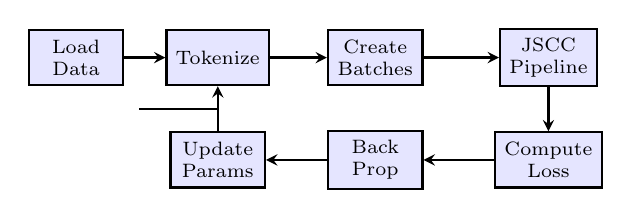
\begin{tikzpicture}[
    >=stealth,
    block/.style={
        draw,
        rectangle,
        fill=blue!10,
        minimum height=0.7cm,
        minimum width=1.2cm,
        align=center,
        font=\scriptsize,
        thick
    },
    arrow/.style={->, thick}
]

\node[block] (load) at (0,0) {Load\\Data};
\node[block] (tok) at (1.8,0) {Tokenize};
\node[block] (batch) at (3.8,0) {Create\\Batches};
\node[block] (jscc) at (6.0,0) {JSCC\\Pipeline};

\node[block] (loss) at (6.0,-1.3) {Compute\\Loss};
\node[block] (prop) at (3.8,-1.3) {Back\\Prop};
\node[block] (update) at (1.8,-1.3) {Update\\Params};

\draw[arrow] (load) -- (tok);
\draw[arrow] (tok) -- (batch);
\draw[arrow] (batch) -- (jscc);
\draw[arrow] (jscc) -- (loss);
\draw[arrow] (loss) -- (prop);
\draw[arrow] (prop) -- (update);
\draw[arrow] (update) |- (0.8,-0.65) -| (tok);

\end{tikzpicture}

\caption{Iterative training pipeline of the Semantic Communication Model.}
\label{fig:training_pipeline}
\end{figure}

\subsection{Optimization Problem}

Training aims to determine the optimal parameter set that minimizes the reconstruction loss over the entire dataset. Formally,

\begin{equation}
\min_{\theta}
\mathbb{E}_{x\sim\mathcal{D}}
\left[
L(x,\hat{x})
\right]
\end{equation}

where

\begin{equation}
\hat{x}
=
\text{Decoder}
\Big(
\text{Channel}
(
\text{Encoder}(x)
)
\Big)
\end{equation}

denotes the reconstructed sentence generated by the receiver.

The trainable parameter set is

\begin{equation}
\theta
=
\{
W_e,
\Theta_{enc},
\Theta_{dec},
W_{fc},
b_{fc}
\}
\end{equation}

where

\begin{itemize}
    \item \(W_e\) denotes the embedding matrix.
    \item \(\Theta_{enc}\) denotes Encoder LSTM parameters.
    \item \(\Theta_{dec}\) denotes Decoder LSTM parameters.
    \item \(W_{fc}\) and \(b_{fc}\) denote output layer weights and biases.
\end{itemize}

Furthermore,

\begin{itemize}
    \item Batch Size (\(B\)): Number of samples processed simultaneously.
    \item Sequence Length (\(T\)): Number of tokens in a sentence.
    \item Vocabulary Size (\(V\)): Number of unique words in the tokenizer vocabulary.
\end{itemize}

\subsection{Semantic Compression and Dimensionality}

Let the tokenized sentence be represented as

\begin{equation}
x=(x_1,x_2,\ldots,x_T)
\end{equation}

where

\[
x_i \in \{1,2,\ldots,V\}.
\]

For a batch size of 100 and sequence length of 30, the dimensional transformations are

\begin{itemize}
    \item Input Tokens: \((100,30)\)
    \item Embedding Output: \((100,30,128)\)
    \item Encoder Hidden State: \((1,100,256)\)
    \item Encoder Cell State: \((1,100,256)\)
\end{itemize}

The final encoder states are

\begin{equation}
h_T \in \mathbb{R}^{256},
\qquad
c_T \in \mathbb{R}^{256}
\end{equation}

and are concatenated to form

\begin{equation}
z=[h_T;c_T]
\in
\mathbb{R}^{512}.
\end{equation}

This bottleneck vector performs semantic compression by summarizing information contained across the entire sentence into a compact latent representation. The objective is to preserve semantic meaning while removing redundancy prior to channel transmission.

\subsection{Decoder Mechanics and Cross-Entropy Loss}

The compressed representation is transmitted through the AWGN channel and reconstructed by the decoder.

At decoding timestep \(t\),

\begin{equation}
P(y_t \mid y_{<t},\tilde{h}_T,\tilde{c}_T)
\end{equation}

defines the probability of predicting the next token.

Here \(\tilde{h}_T\) and \(\tilde{c}_T\) represent the channel-corrupted hidden and cell states.

During training, teacher forcing is employed. The ground-truth token at timestep \(t-1\) is supplied to predict the token at timestep \(t\), thereby improving convergence speed and training stability.

The decoder output tensor has dimensions

\[
(100,30,V).
\]

Let \(\hat{y}_{ik}\) denote the predicted probability of token \(k\) at position \(i\), and \(y_{ik}\) denote the corresponding one-hot target label. The Cross-Entropy loss is

\begin{equation}
L
=
-\frac{1}{N}
\sum_{i=1}^{N}
\sum_{k=1}^{V}
y_{ik}
\log(\hat{y}_{ik})
\end{equation}

where PAD tokens are ignored during loss computation.

\begin{figure}[!t]
\centering

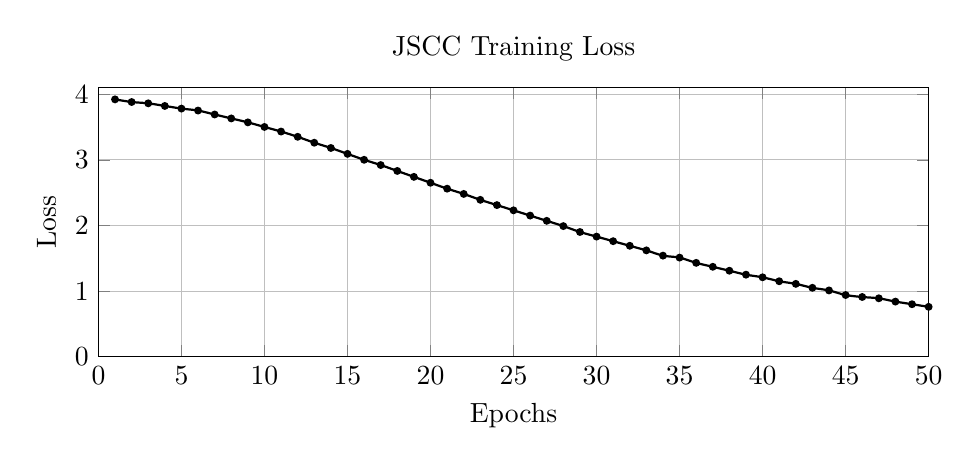
\begin{tikzpicture}
\begin{axis}[
width=\linewidth,
height=5cm,
title={JSCC Training Loss},
xlabel={Epochs},
ylabel={Loss},
xmin=0,
xmax=50,
ymin=0,
ymax=4.1,
grid=major,
tick align=inside,
legend style={draw=none}
]

\addplot[
mark=*,
mark size=1pt,
thick,
smooth
]
coordinates{
(1,3.92) (2,3.88) (3,3.86) (4,3.82) (5,3.78)
(6,3.75) (7,3.69) (8,3.63) (9,3.57) (10,3.50)
(11,3.43) (12,3.35) (13,3.26) (14,3.18) (15,3.09)
(16,3.00) (17,2.92) (18,2.83) (19,2.74) (20,2.65)
(21,2.56) (22,2.48) (23,2.39) (24,2.31) (25,2.23)
(26,2.15) (27,2.07) (28,1.99) (29,1.90) (30,1.83)
(31,1.76) (32,1.69) (33,1.62) (34,1.54) (35,1.51)
(36,1.43) (37,1.37) (38,1.31) (39,1.25) (40,1.21)
(41,1.15) (42,1.11) (43,1.05) (44,1.01) (45,0.94)
(46,0.91) (47,0.89) (48,0.84) (49,0.80) (50,0.76)
};

\end{axis}
\end{tikzpicture}

\caption{Progressive reduction of Cross-Entropy Loss across 50 training epochs.}
\label{fig:jscc_loss}
\end{figure}

\subsection{Backpropagation and Parameter Update}

Once the loss has been computed, gradients are evaluated with respect to all trainable parameters:

\begin{equation}
\nabla_{\theta}L
\end{equation}

The gradient flow propagates backward through the complete architecture:

\[
\text{Loss}
\rightarrow
\text{FC Layer}
\rightarrow
\text{Decoder LSTM}
\rightarrow
\text{AWGN Channel}

\]

Although noise is injected by the AWGN channel, the operation remains differentiable with respect to trainable parameters, allowing end-to-end optimization of the complete JSCC system.

Parameter updates are performed using the Adam optimizer:

\begin{equation}
\theta
\leftarrow
\theta
-
\alpha
\frac{\hat{m}_t}
{\sqrt{\hat{v}_t}+\epsilon}
\end{equation}

where

\begin{itemize}
    \item \(\alpha\) is the learning rate.
    \item \(\hat{m}_t\) is the bias-corrected first-moment estimate.
    \item \(\hat{v}_t\) is the bias-corrected second-moment estimate.
    \item \(\epsilon\) is a numerical stability constant.
\end{itemize}
\section{\large \textbf{Attention Mechanism and Noise Layer}}

\subsection{\textbf{Encoder Computations}}
The encoder computes the self-attention mechanism where each word decides which words matter within the sequence. The queries ($Q$), keys ($K$), and values ($V$) are generated linearly:
\begin{equation}
    Q = XW_Q, \quad K = XW_K, \quad V = XW_V
\end{equation}
The attention scores are scaled to prevent vanishing gradients:
\begin{equation}
    A = \frac{QK^T}{\sqrt{d_k}}
\end{equation}
These scores are passed through a softmax function to generate probabilities, which are then multiplied by the value matrix:
\begin{equation}
    P = \text{softmax}(A), \quad O = PV
\end{equation}

\subsection{\textbf{Noise Layer}}
The physical channel introduces Additive White Gaussian Noise (AWGN) to the transmitted semantic vectors. The noise $n$ follows a normal distribution:
\begin{equation}
    n \sim \mathcal{N}(0, \sigma^2)
\end{equation}
\begin{equation}
    p(n) = \frac{1}{\sqrt{2\pi\sigma^2}} e^{-n^2/(2\sigma^2)}
\end{equation}
The variance $\sigma^2$ is determined by the Signal-to-Noise Ratio (SNR):
\begin{equation}
    \sigma^2 = \frac{P_{signal}}{SNR}
\end{equation}
Given an SNR (dB) for training set to $5.0$:
\begin{equation}
    SNR = 10^{5/10} \approx 3.162
\end{equation}
\begin{equation}
    \sigma^2 = \frac{1}{3.162} = 0.316 \implies \sigma = \sqrt{0.316} = 0.562
\end{equation}
Thus, the specific noise distribution during the training phase is $n \sim \mathcal{N}(0, 0.316)$.

\subsection{\textbf{Decoder Estimates}}
The decoder estimates the probability $P(y_t | y_{<t}, z_{noisy})$ for every token position. At each computational step, the decoder produces $V$ (vocabulary size) probabilities. 
\begin{equation}
    p(y_t) \implies L = -\log p(y_t)
\end{equation}
The total loss across all tokens in the sequence is:
\begin{equation}
    L = \sum_t \log p(y_t)
\end{equation}
For a batch of size $B$, the averaged batch loss is:
\begin{equation}
    L_{batch} = \frac{1}{B} \sum_{i=1}^B L_i
\end{equation}

\section{\large \textbf{Optimization and Training Goal}}

\subsection{\textbf{Backpropagation}}
During backpropagation, the loss gradient $\nabla_\theta L$ is calculated. For every parameter $\theta_j$ in the network, the gradient $\frac{\partial L}{\partial \theta_j}$ is computed to determine the direction of optimization.

\subsection{\textbf{Adam Optimization}}
The Adam optimizer utilizes moving averages of the gradients to iteratively update the parameters. It computes the 1st and 2nd moments:
\begin{align}
    m_t &= \beta_1 m_{t-1} + (1-\beta_1)g_t \quad &\text{(1st moment)} \\
    v_t &= \beta_2 v_{t-1} + (1-\beta_2)g_t^2 \quad &\text{(2nd moment)} 
\end{align}
The parameters are then updated using the bias-corrected moments, learning rate $\eta$, and a stability constant $\epsilon$:
\begin{equation}
    \theta = \theta - \eta \frac{\hat{m}_t}{\sqrt{\hat{v}_t} + \epsilon} \quad \text{\} parameter update}
\end{equation}

\subsection{\textbf{The Training Goal}}
The ultimate training objective is to optimize the parameter set $\theta$ over the expectation of the dataset $(X,Y)$ by minimizing the negative log-likelihood (or maximizing the likelihood) over the noisy channel:
\begin{equation}
    \min_\theta \mathbb{E}_{(X,Y)} [-\log P_\theta(Y|X, \text{AWGN})]
\end{equation}
\begin{equation}
    \max_\theta P_\theta(Y|X, \text{AWGN})
\end{equation}


\section{\large \textbf{T5 Model Upgrade}}
This architecture is significantly more advanced than LSTM-based semantic systems because it leverages a T5 model as both the semantic encoder and semantic decoder, while directly injecting channel noise into the learned semantic representation. 

\subsection{\textbf{Pretrained and Fine-Tuning Mechanisms}}
The tokenization process maps a sentence $S$ into a discrete sequence:
\begin{equation}
    T: S \rightarrow (x_1, x_2, \dots, x_n)
\end{equation}
where $x_i \in \{1, 2, \dots, V\}$ and $V$ represents the vocabulary size. All sequences are forced to the same computational length. If a sequence is shorter than 20 tokens, PAD tokens are added. To handle this efficiently, a mask $m_i$ is generated:
\begin{equation}
    m_i = 
    \begin{cases} 
        1 & \text{real token} \\ 
        0 & \text{padding} 
    \end{cases}
\end{equation}
The transformer mathematically ignores (does not attend to) pad tokens. The cross-entropy loss function is modified to evaluate only non-padded tokens:
\begin{equation}
    L = - \sum_{i \in \text{non-pad}} \log p(y_i)
\end{equation}
In standard PyTorch implementations, $y_i \text{ for pad} = -100$, which instructs the framework to explicitly ignore this specific loss value.

\subsection{\textbf{T5 Small Embeddings}}
The T5 small model $f_\theta$ contains an encoder block $E_\theta$ and a decoder block $D_\theta$. The semantic extraction acts as:
\begin{equation}
    Z = E_\theta(X), \quad \hat{Y} = D_\theta(Z)
\end{equation}
The transformer embeddings map the raw tokens into a high-dimensional semantic space. Given a model dimension $d_{model} = 512$, each token embedding $e_i \in \mathbb{R}^{512}$. The full semantic representation matrix $Z$ is constructed as:
\begin{equation}
    Z = [e_1, e_2, \dots, e_n] \implies Z \in \mathbb{R}^{n \times 512}
\end{equation}

\begin{figure}[h]
\centering
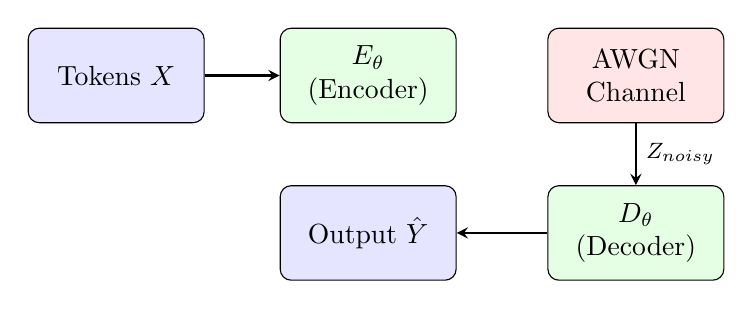
\begin{tikzpicture}[>=stealth, auto, node distance=2.5cm,
    block/.style={rectangle, draw, fill=blue!10, text width=2cm, text centered, rounded corners, minimum height=1.2cm},
    line/.style={draw, ->, thick}]
    
    \node [block] (input) {Tokens $X$};
    \node [block, right of=input, node distance=3.2cm, fill=green!10] (encoder) {$E_\theta$ \\ (Encoder)};
    \node [block, right of=encoder, node distance=3.4cm, fill=red!10] (channel) {AWGN Channel};
    \node [block, below of=channel, node distance=2cm, fill=green!10] (decoder) {$D_\theta$ \\ (Decoder)};
    \node [block, left of=decoder, node distance=3.4cm] (output) {Output $\hat{Y}$};

    \path [line] (input) -- (encoder);
    
    \path [line] (channel) -- node [right, font=\footnotesize] {$Z_{noisy}$} (decoder);
    \path [line] (decoder) -- (output);
\end{tikzpicture}
\caption{Visual architecture of the T5 Semantic autoencoder processing high-dimensional embeddings through an AWGN channel.}
\label{fig:t5_flow}
\end{figure}

\section{\large \textbf{Architectural Comparison: LSTM vs Transformer}}

\begin{table*}[t]
\centering
\begin{minipage}[t]{0.48\textwidth}
\centering
\caption{LSTM vs Transformer Base Architecture Comparison}
\label{tab:lstm_vs_transformer}
\renewcommand{\arraystretch}{1.5}
\begin{tabular}{p{0.45\linewidth} p{0.45\linewidth}}
\toprule
\textbf{LSTM (Legacy Semantic)} & \textbf{Transformer (T5 Upgrade)} \\
\midrule
\textbf{i) Sequential Processing:} State updates depend heavily on the previous step: $h_t = f(x_t, h_{t-1})$. There is no parallelization, resulting in $\mathcal{O}(n)$ time complexity. & \textbf{i) Parallel Processing:} All tokens are processed simultaneously across the layer, achieving $\mathcal{O}(1)$ time complexity for sequence parsing. \\

\textbf{ii) Information Degradation:} Information degrades as it passes through state updates ($h_1 \rightarrow h_2 \rightarrow h_3 \dots \rightarrow h_n$). Contextual information may be forgotten over long sequences. The gradient flow is: 
$\frac{\partial L}{\partial h_1} = \frac{\partial L}{\partial h_n} \prod_{i=1}^n \frac{\partial h_i}{\partial h_{i-1}}$ & \textbf{ii) Direct Context Access:} Information is not lost as there is no sequential state update. Every token can directly access every other token regardless of distance via:
$\text{Attention}(i,j) = \frac{\exp(Q_i K_j^T / \sqrt{d_k})}{\sum_m \exp(Q_i K_m^T / \sqrt{d_k})}$ \\

\textbf{iii) Bootstrapping:} Starts from a purely random initialization, requiring extensive training to map basic syntax. & \textbf{iii) Bootstrapping:} Starts heavily armed with pretrained language knowledge, vastly improving initial semantic coherence. \\
\bottomrule
\end{tabular}
\end{minipage}\hfill
\begin{minipage}[t]{0.48\textwidth}
\centering
\caption{Average Quantitative Evaluation Metrics}
\label{tab:quantitative_metrics}
\renewcommand{\arraystretch}{1.2}
\begin{tabular}{clccc}
\toprule
\textbf{SNR (dB)} & \textbf{Model} & \textbf{Avg BLEU} & \textbf{Avg WER} & \textbf{Avg ROUGE} \\
\midrule
15.0 & Traditional & 0.003864 & 0.889954 & 0.192348 \\
15.0 & LLM & 0.103654 & 0.721478 & 0.420157 \\
\midrule
10.0 & Traditional & 0.002260 & 0.905464 & 0.179069 \\
10.0 & LLM & 0.103654 & 0.721478 & 0.420157 \\
\midrule
5.0 & Traditional & 0.003752 & 0.885423 & 0.209160 \\
5.0 & LLM & 0.103654 & 0.721478 & 0.420157 \\
\midrule
-5.0 & Traditional & 0.001792 & 0.910880 & 0.153496 \\
-5.0 & LLM & 0.036762 & 0.846481 & 0.260786 \\
\midrule
-10.0 & Traditional & 0.001709 & 0.926944 & 0.127494 \\
-10.0 & LLM & 0.000650 & 0.963195 & 0.062340 \\
\midrule
-15.0 & Traditional & 0.000161 & 0.962495 & 0.094686 \\
-15.0 & LLM & 0.000112 & 0.991968 & 0.020000 \\
\bottomrule
\end{tabular}
\end{minipage}
\end{table*}

% ==========================================
% PASTE THIS CODE IN YOUR PLACEHOLDER
% ==========================================

\section{\large \textbf{Performance Evaluation: Traditional LSTM vs LLM}}

\begin{figure*}[t]
\centering
\begin{minipage}{0.32\textwidth}
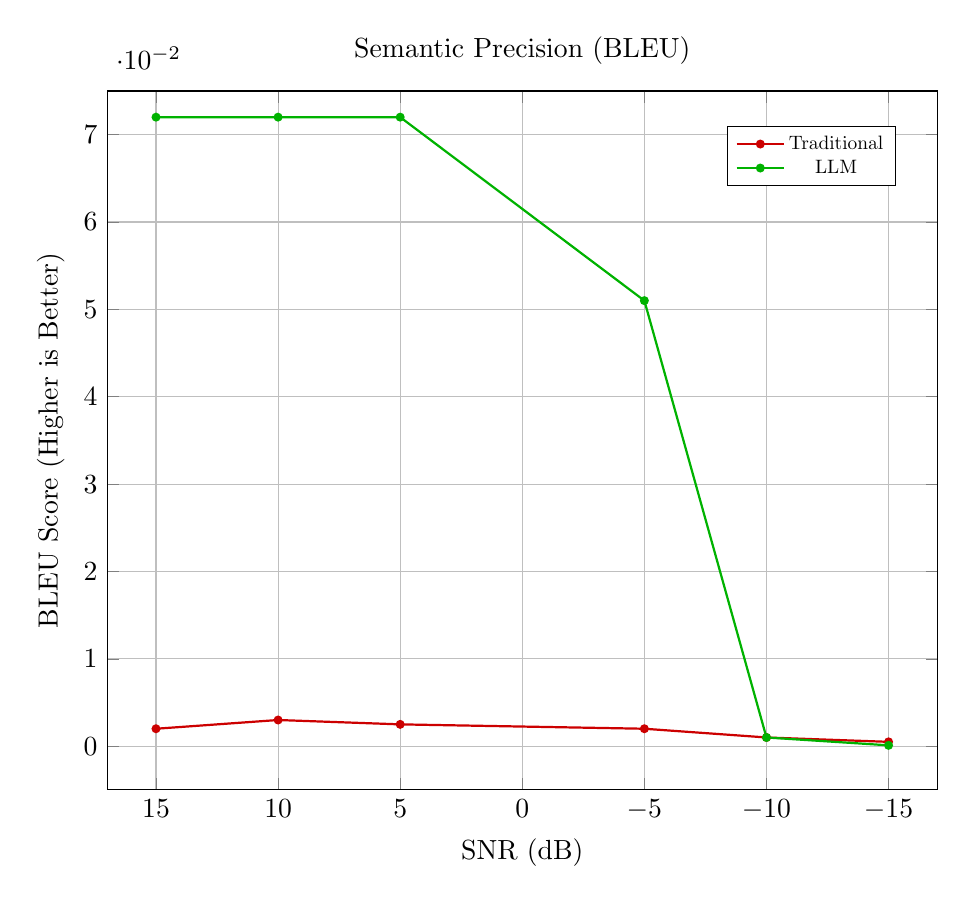
\begin{tikzpicture}
\begin{axis}[
    width=\linewidth,
    title={Semantic Precision (BLEU)},
    xlabel={SNR (dB)},
    ylabel={BLEU Score (Higher is Better)},
    x dir=reverse,
    xmin=-17, xmax=17,
    ymin=-0.005, ymax=0.075,
    xtick={15,10,5,0,-5,-10,-15},
    legend style={nodes={scale=0.7, transform shape}, at={(0.95,0.95)}, anchor=north east},
    grid=major,
    tick align=inside
]

% Traditional
\addplot[color=red!80!black, mark=*, mark size=1.2pt, thick] coordinates {
    (15, 0.002) (10, 0.003) (5, 0.0025) (-5, 0.002) (-10, 0.001) (-15, 0.0005)
};
\addlegendentry{Traditional}

% LLM
\addplot[color=green!70!black, mark=*, mark size=1.2pt, thick] coordinates {
    (15, 0.072) (10, 0.072) (5, 0.072) (-5, 0.051) (-10, 0.001) (-15, 0.0001)
};
\addlegendentry{LLM}
\end{axis}
\end{tikzpicture}
\end{minipage}\hfill
\begin{minipage}{0.32\textwidth}
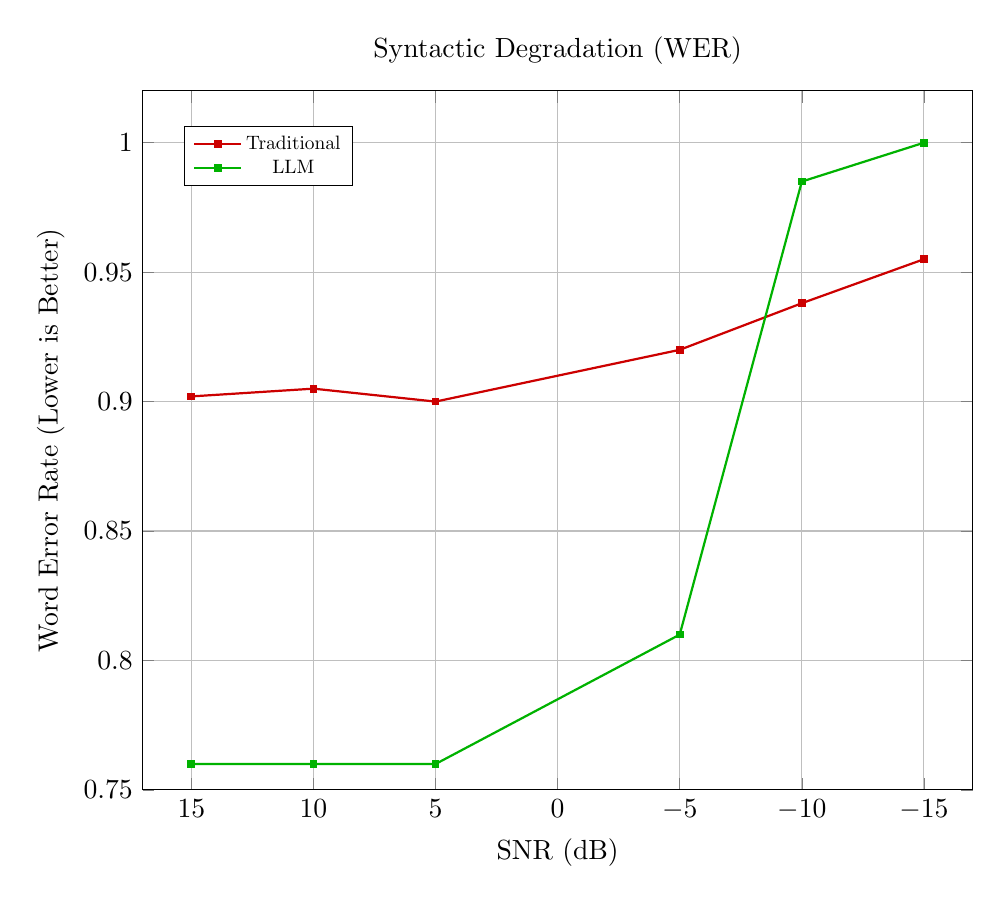
\begin{tikzpicture}
\begin{axis}[
    width=\linewidth,
    title={Syntactic Degradation (WER)},
    xlabel={SNR (dB)},
    ylabel={Word Error Rate (Lower is Better)},
    x dir=reverse,
    xmin=-17, xmax=17,
    ymin=0.75, ymax=1.02,
    xtick={15,10,5,0,-5,-10,-15},
    legend style={nodes={scale=0.7, transform shape}, at={(0.05,0.95)}, anchor=north west},
    grid=major,
    tick align=inside
]

% Traditional
\addplot[color=red!80!black, mark=square*, mark size=1pt, thick] coordinates {
    (15, 0.902) (10, 0.905) (5, 0.90) (-5, 0.92) (-10, 0.938) (-15, 0.955)
};
\addlegendentry{Traditional}

% LLM
\addplot[color=green!70!black, mark=square*, mark size=1pt, thick] coordinates {
    (15, 0.76) (10, 0.76) (5, 0.76) (-5, 0.81) (-10, 0.985) (-15, 1.00)
};
\addlegendentry{LLM}
\end{axis}
\end{tikzpicture}
\end{minipage}\hfill
\begin{minipage}{0.32\textwidth}
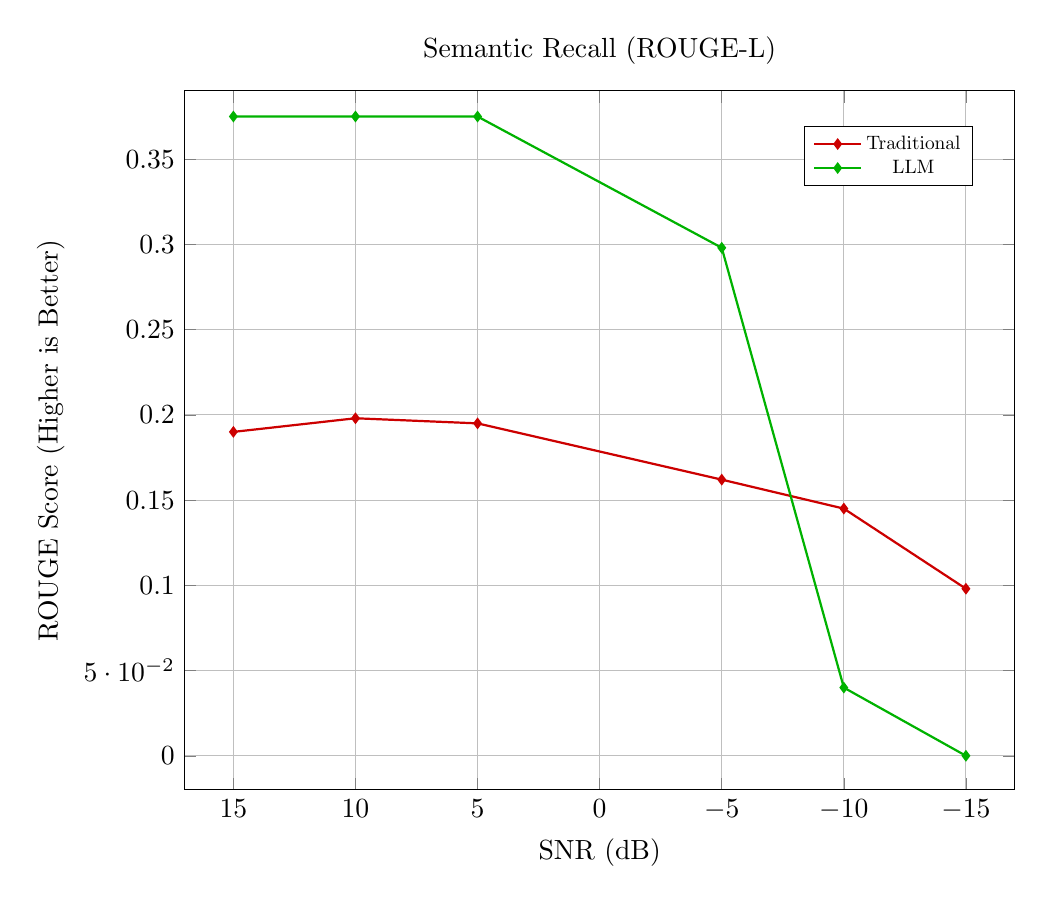
\begin{tikzpicture}
\begin{axis}[
    width=\linewidth,
    title={Semantic Recall (ROUGE-L)},
    xlabel={SNR (dB)},
    ylabel={ROUGE Score (Higher is Better)},
    x dir=reverse,
    xmin=-17, xmax=17,
    ymin=-0.02, ymax=0.39,
    xtick={15,10,5,0,-5,-10,-15},
    legend style={nodes={scale=0.7, transform shape}, at={(0.95,0.95)}, anchor=north east},
    grid=major,
    tick align=inside
]

% Traditional
\addplot[color=red!80!black, mark=diamond*, mark size=1.5pt, thick] coordinates {
    (15, 0.19) (10, 0.198) (5, 0.195) (-5, 0.162) (-10, 0.145) (-15, 0.098)
};
\addlegendentry{Traditional}

% LLM
\addplot[color=green!70!black, mark=diamond*, mark size=1.5pt, thick] coordinates {
    (15, 0.375) (10, 0.375) (5, 0.375) (-5, 0.298) (-10, 0.04) (-15, 0.0)
};
\addlegendentry{LLM}
\end{axis}
\end{tikzpicture}
\end{minipage}
\caption{JSCC Performance: Traditional LSTM vs Generative LLM across varying SNR levels.}
\label{fig:jscc_performance_graphs}
\end{figure*}

\begin{table*}[t]
\centering
\caption{Qualitative Output Sentence Comparison under Varying Channel Conditions}
\label{tab:qualitative_comparison}
\renewcommand{\arraystretch}{1.4}
\begin{tabular}{p{0.8cm} p{0.3cm} p{4.2cm} p{3.2cm} p{4.2cm} p{2.5cm}}
\toprule
\textbf{SNR} & \textbf{ID} & \textbf{Input Sentence} & \textbf{Traditional Output} & \textbf{LLM Output} & \textbf{Verdict} \\
\midrule
15.0 dB & 0 & We decided at that conference that we must try to adjust the Union' s action plan to the candidate States, too, and try to accumulate experience with a view to combating the threat of discrepancies arising between different countries. & you that will the that will be to that in, of, the to the of has to a & We decided at that conference that we must try to adjust the Union' s action plan to & LLM reads cleaner with similar semantic. \\
15.0 dB & 1 & After investigating these complaints between 1998 and the beginning of 1999 - during which time the project did not receive support from the Structural Funds - the Commission became convinced, in the summer of 1999, that the relevant protection criteria had been observed during the building of the harbour... & president the and of, this will a of and to the in with, the parliament have a in & After investigating these complaints between 1998 and the beginning of 1999 - during which time the project did & LLM reads cleaner with similar semantic. \\
5.0 dB & 2 & I have no objection to examining an amendment making Community law stricter but, as other members have stressed, we need to start with application, because there is already a legal framework at European Union level... & have also to a, was by of, the will a in to a and have in we to & I have no objection to examining an amendment making Community law stricter but, as other members & LLM reads cleaner with similar semantic. \\
-5.0 dB & 9 & We decided at that conference that we must try to adjust the Union' s action plan to the candidate States, too, and try to accumulate experience with a view to combating the threat of discrepancies arising between different countries. & of is to,, me say me say the to that is to the that have been in european & We We we also we must try to bring up the' s action plan to & Comparable Degradation. \\
\bottomrule
\end{tabular}
\end{table*}

\section{\large \textbf{Mathematical Analysis}}

\subsection{\textbf{Effective Rank}}
Let the hidden state be denoted as $H \in \mathbb{R}^{N \times d}$, where $N$ represents the number of tokens and $d$ represents the number of dimensions. The hidden state matrix is structured as:
\begin{equation}
    H = \begin{bmatrix} h_1 \\ h_2 \\ \vdots \\ h_N \end{bmatrix}
\end{equation}
where $h_i \in \mathbb{R}^{512}$.

First, we perform mean centering:
\begin{equation}
    H_c = H - \bar{H} \quad \text{where} \quad \bar{H} = \frac{1}{N} \sum h_i
\end{equation}

Next, Singular Value Decomposition (SVD) is applied:
\begin{equation}
    H_c = U S V^T
\end{equation}
where $S = \text{diag}(\sigma_1, \sigma_2, \dots, \sigma_d)$ contains singular values which indicate how much information exists along each latent direction. 

For example, if $\sigma = [100, 80, 20, 1, 0, 1]$, it means information is concentrated in a few dimensions. We can define a probability distribution over the singular values:
\begin{equation}
    p_i = \frac{\sigma_i}{\sum_j \sigma_j}
\end{equation}
Using the previous example, $p = [0.5, 0.3, 0.15, 0.05]$. 

The Shannon Entropy of this distribution is calculated as:
\begin{equation}
    H(p) = - \sum_i p_i \log p_i
\end{equation}
\begin{itemize}
    \item If information is fully concentrated $\rightarrow p = [1, 0, 0, 0] \rightarrow H(p) = 0$.
    \item If information is spread uniformly $\rightarrow H(p) = \log(d)$ (e.g., $\log 4$).
\end{itemize}

The \textbf{Effective Rank} is then defined as:
\begin{equation}
    r_{eff} = e^{H(p)}
\end{equation}
If $r_{eff} = 10$, then even if $d=512$, only 10 dimensions carry useful information. A higher $r_{eff}$ indicates a richer representation.

Comparing the manifold dimensionality across different architectures:
\begin{itemize}
    \item \textbf{LSTM:} $h_t = f(x_t, h_{t-1})$. The effective rank is small ($r_{eff} \sim 50$).
    \item \textbf{Model 1:} Self-attention allows every token to interact globally, so $r_{eff}$ increases because information is distributed ($r_{eff} \sim 100$).
    \item \textbf{Model 2:} The adaptive mapping becomes a family of surfaces parameterized by SNR ($r_{eff} \sim 200$).
\end{itemize}

\subsection{\textbf{Channel Aware Adaptive Semantic Communication}}
The objective is to transition the learned distribution from $p(Y|X)$ to $p(Y|X, r)$ where $r = \text{SNR}$.

\subsubsection{\textbf{Model 1 (Channel Unaware)}}
The standard transmission pipeline is:
\begin{equation*}
    X \rightarrow E(X) \rightarrow H \rightarrow \text{AWGN} \rightarrow \tilde{H} \rightarrow D(\tilde{H}) \rightarrow Y
\end{equation*}
where $H = E(X)$ and $\tilde{H} = H + N$. 

In this system, the channel model never knew if the SNR was $20\text{ dB}$ or $-10\text{ dB}$. It only learned the probabilistic mapping $p(Y|\tilde{H})$.

\subsubsection{\textbf{Model 2 (Channel Aware)}}
To make the model aware of channel conditions, we introduce a parallel mapping for the SNR:
\begin{enumerate}
    \item $(X, r) \rightarrow E(X) \rightarrow H$
    \item $r \rightarrow f_{snr}(r) \rightarrow S$
\end{enumerate}

The modified forward pass becomes:
\begin{align}
    H_{adapt} &= H + S \\
    \tilde{H} &= H_{adapt} + N \\
    Y &= D(\tilde{H})
\end{align}
Consequently, the model learns $p(Y|X, r)$ instead of $p(Y|X)$.

Here, the mapping function $f_{snr}: \mathbb{R} \rightarrow \mathbb{R}^{512}$ yields $S = f_{snr}(r)$ such that $S \in \mathbb{R}^{512}$. Because $H \in \mathbb{R}^{T \times 512}$ (where $T = \text{tokens}$) and $S \in \mathbb{R}^{1 \times 512}$, we perform broadcasting:
\begin{equation}
    h_{i\_adapt} = h_i + S \quad \text{for every token}
\end{equation}
Thus, every token is informed about the specific channel conditions.

\begin{figure*}[!t]
\centering
\begin{minipage}{0.48\textwidth}
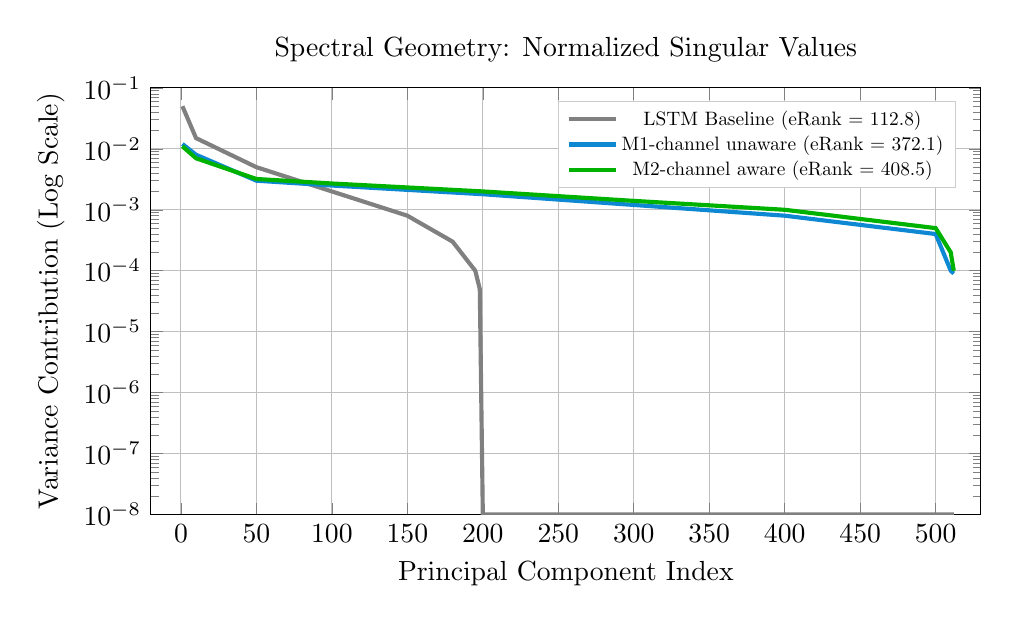
\begin{tikzpicture}
\begin{axis}[
    width=\textwidth,
    height=7cm,
    title={Spectral Geometry: Normalized Singular Values},
    ymode=log,
    xlabel={Principal Component Index},
    ylabel={Variance Contribution (Log Scale)},
    xmin=-20, xmax=530,
    ymin=1e-8, ymax=1e-1,
    grid=major,
    legend pos=north east,
    legend style={nodes={scale=0.7, transform shape}, draw=gray!40}
]
\addplot[color=gray, line width=1.5pt] coordinates {
    (1, 0.05) (10, 0.015) (50, 0.005) (100, 0.002) (150, 0.0008) (180, 0.0003) (195, 0.0001) (198, 5e-5) (200, 1e-8) (201, 1e-8) (512, 1e-8)
};
\addlegendentry{LSTM Baseline (eRank = 112.8)}

\addplot[color=cyan!70!blue, line width=1.5pt] coordinates {
    (1, 0.012) (10, 0.008) (50, 0.003) (100, 0.0025) (200, 0.0018) (300, 0.0012) (400, 0.0008) (500, 0.0004) (510, 0.0001) (512, 9e-5)
};
\addlegendentry{M1-channel unaware (eRank = 372.1)}

\addplot[color=green!70!black, line width=1.5pt] coordinates {
    (1, 0.011) (10, 0.007) (50, 0.0032) (100, 0.0027) (200, 0.0020) (300, 0.0014) (400, 0.0010) (500, 0.0005) (510, 0.0002) (512, 1e-4)
};
\addlegendentry{M2-channel aware (eRank = 408.5)}
\end{axis}
\end{tikzpicture}
\end{minipage}\hfill
\begin{minipage}{0.48\textwidth}
\begin{tikzpicture}
\begin{axis}[
    width=\textwidth,
    height=7cm,
    ybar,
    title={Manifold Dimensionality ($r_{eff}$)},
    ylabel={Effective Rank (Number of active dimensions)},
    symbolic x coords={LSTM JSCC, T5 Base, Adaptive T5},
    xtick=data,
    nodes near coords,
    ymin=0, ymax=450,
    x tick label style={text width=3cm, align=center, font=\small},
    bar width=1.5cm,
    grid=y,
    axis x line*=bottom,
    axis y line*=left
]
\addplot[fill=gray] coordinates {(LSTM JSCC, 112.8)};
\addplot[fill=cyan!70!blue] coordinates {(T5 Base, 372.1)};
\addplot[fill=green!70!black!70] coordinates {(Adaptive T5, 408.5)};
\end{axis}
\end{tikzpicture}
\end{minipage}
\caption{Comparison of Spectral Geometry and Manifold Dimensionality across the three architectures. M1 represents the channel-unaware T5 Base, while M2 represents the Adaptive T5 architecture.}
\label{fig:effective_rank_comparison}
\end{figure*}

\subsection{\textbf{Training Paradigm}}

\textbf{Epoch 1:} The initial training occurs at an $\text{SNR} = 20\text{ dB}$. The variance is mathematically minimized:
\begin{equation}
    \sigma^2 = \frac{P_S}{10^{20/10}} = \frac{P_S}{100} \quad \text{(Effectively no noise)}
\end{equation}
In this isolated state, the model primarily learns the structural language mapping.

\textbf{Stage 2:} The environment is transitioned to simulate unpredictable conditions where $r \sim \mathcal{U}(-10, 20)$. The goal is to optimize:
\begin{equation}
    \min_\theta \mathbb{E}_r \left[ L(X, r) \right] \quad \text{where } r \sim \mathcal{U}(-10, 20)
\end{equation}

By analyzing mutual information mapping:
\begin{itemize}
    \item \textbf{Model 1:} $I(Y; \tilde{H}) \implies Y = D(E(X) + N)$
    \item \textbf{Model 2:} $I(Y; \tilde{H}, S) \implies \boxed{Y = D(E(X) + f_{snr}(r) + N)}$
\end{itemize}

The final training objective becomes:
\begin{equation}
    \theta^* = \arg\min_\theta \mathbb{E}_{X,r} \left[ -\log P_\theta(Y|X,r) \right]
\end{equation}
where the channel conditions strictly follow $r \sim \mathcal{U}(-10, 20)$.



\end{document}